\documentclass[UTF8,10pt,a4paper]{ctexart}
\usepackage[utf8]{inputenc}
\usepackage{amsmath}
\usepackage{amsfonts}
\usepackage{amssymb}
\usepackage{graphicx}

\author{陈斯杰}
\title{Chapter1. THE GENESIS OF FOURIER ANALYSIS}
\begin{document}
\maketitle
\begin{abstract}
This book begins the talk of Fourier Analysis with two 
physical problem: vibrating string and heat conduction.
In this review, I am going to illustrate these two examples
in detail by supplementing the background knowledge.
\end{abstract}

\section{The Vibrating String}
	\subsection{Simple harmonic motion 简谐运动}
		\begin{figure}[ht]
			\centering
			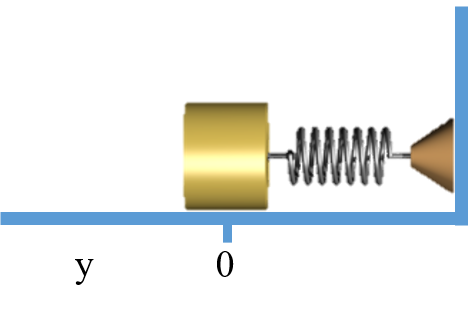
\includegraphics[width=5cm]{idealspring.png}
			\caption{简谐运动谐振子}
			\label{fig:xiantu}
		\end{figure}
		
		\noindent
		Newton's law produces a 2nd order ODE

		\begin{equation}
			F=-ky(t) \Rightarrow -ky(t)=my''(t)
		\end{equation}

		Let $c=\sqrt{\frac{k}{m}}$, we get a neater form: 
		
		\begin{equation}
			y''(t)+c^2y(t)=0
		\end{equation}				
		\noindent
		Equation(2)	is a linear homogeneous 2nd-order differential equation(二阶常系数线性方程).
		For a general case $y''+py'+qy=0$, we first solve the characteristic equation
		$\lambda^2+p\lambda+q=0$ and get the characteristic roots: $\lambda_1, \lambda_2$.
		
		\begin{tabular}{|lll|}
		\hline
		Characteristic Roots & Linear Independent Sol. Pair & General Sol.\\
		\hline
		$\lambda_1,\lambda_2\in\mathbb{R}\ and\ \lambda_1\neq\lambda_2$ &
		$y_1=e^{\lambda_1 x}, y_2=e^{\lambda_2 x}$ &
		$y=C_1e^{\lambda_1 x}+C_2e^{\lambda_2 x}$ \\
		
		$\lambda_1,\lambda_2\in\mathbb{R}\ and\ \lambda_1=\lambda_2$ &
		$y_1=e^{\lambda_1 x}, y_2=xe^{\lambda_1 x}$ &
		$y=(C_1+C_2x)e^{\lambda_1 x}$ \\
		
		$\lambda_1,\lambda_2=\alpha\pm i\beta$ &
		$y_1=e^{\alpha x}\cos\beta x, y_2=e^{\alpha x}\sin\beta x$ &
		$y=e^{\alpha x}(C_1 \cos\beta x +C_2 \sin\beta x)$ \\
		\hline
		\end{tabular}
    	\  \\
		The corresponding characteristic equation of (2) is $\lambda^2 + c^2=0$, and the roots
		are $\lambda=\pm ic$; therefore, the general solution of (2) is 
		\begin{equation}
			y(t)=a\cos ct+b\sin ct
		\end{equation}
		and it's 1st order derivative is
		\begin{equation}
			y'(t)=-ac\sin ct +bc\cos ct
		\end{equation}
		To get the particular solution, we need 2 initial condition: $y(0)\ and\ y'(0)$.\\
		$y(0)=a,\ y'(0)=bc$, thereby getting the particular solution:
		\begin{equation}
			y(t)=y'(0)\cos ct + \frac{y'(0)}{c} \sin ct
		\end{equation}
	\subsection{Standing Wave 驻波}
		\begin{figure}[ht]
			\centering
			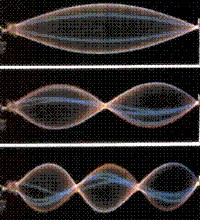
\includegraphics[width=5cm]{standingwave.png}
			\caption{驻波}
			\label{fig:xiantu}
		\end{figure}
		\noindent
		驻波是两个振幅、波长、频率都相同的正弦波,相向而行形成的。
		驻波的波形并不前进,波形上的每个质点皆作Simple Harmonic Motion(简谐运动)。\\
		We use $u(x,t)$ to describe the standing wave. The nature of standing waves suggest 
		the mathematical idea of "separation of variables".\\
		\noindent
		As standing waves do not travel, every mass point just oscillates around the balance position 
		at different amplitudes. So the equation of standing wave movement can be expressed as:
		\begin{equation}
		u(x,t)=\phi (x) \psi(t)
		\end{equation}
		where:\\
		 	$\phi(x)$ represents the amplitute of the mass points at location x. \\
		 	$\psi(t)$ is a oscillating factor, which makes every mass point 
			oscillates within the amplitute $\phi(x)$.
		
		
\end{document}